\chapter{Methodology}

In this chapter, I will describe the decision-making process behind the system used for generating and collecting test data. I will then describe the system itself in more detail.

\section{Background}
The project was initially started by Sintef in collaboration with a company that runs a microservices hosting platform. This company had requested Sintef to do research on their platform, to look at ways to anticipate issues like version conflicts and performance drops. \\
Another student and I were brought onto the project as master thesis project tie-ins. The other student was to focus on technical lag, and I was to focus on performance. However, soon after we had been brought onto the project and gotten the go-ahead from the faculty and everything stamped and sealed, the company that hired Sintef simply stopped responding. No e-mails, no meetings, no phone calls. So we were left stranded, and would have to come up with something for ourselves. \\
We decided to go ahead with the initial goals of the project: To research a microservice system and try to make predictors that could see performance and compatibility issues ahead of time. 
But instead of simply being supplied information about an existing microservice system, we had to create our own systems and our own tests. 

\section{System selection and creation}
Building a microservice system can be a very complex affair, and subject to a master thesis project on its own. So making one from scratch would be far outside the scope of the project. As such, a list of requirements for the project were devised:

\begin{itemize}
    \item The system would need to be relatively quick and easy to get up and running.
    \item It must be possible to generate faults in the system.
    \item The system must be able to collect and provide data about itself and its performance. 
    \item It must be feasible to run and stress test this system on a student's budget.
\end{itemize}

\subsection{Cloud solutions}
Cloud computing is in several ways a natural fit for this project. Microservices as a concept is formulated with cloud computing in mind. Cloud service providers tend to provide some microservice-specific services. 
The three biggest players in cloud services are Amazon, Microsoft and Google \cite*{DgtlInfra}. They all offer some level of free access, and student deals can be negotiated for more credits. They all integrate Kubernetes while adding their own ease-of-use features, so launching some premade system on them should be feasible. \\
However, they come with some issues. The biggest issue is cost. In the course of my work, I was bound to do quite a lot of stress testing. This would be bound to burn through a ton of credits. Another issue would be dealing with their own built-in load balancing and DDoS protection. Getting accurate results from stress testing could turn out expensive as well as unreliable.\\
I set up free accounts for both Google Kubernetes Engine (GKE), Google's distributed cloud service, and Amazon Web Services (AWS), and reached out to apply for a student grant. However, response was slow, and it looked unlikely that I would be granted the necessary amount of credits.

\begin{figure} 
\centering 
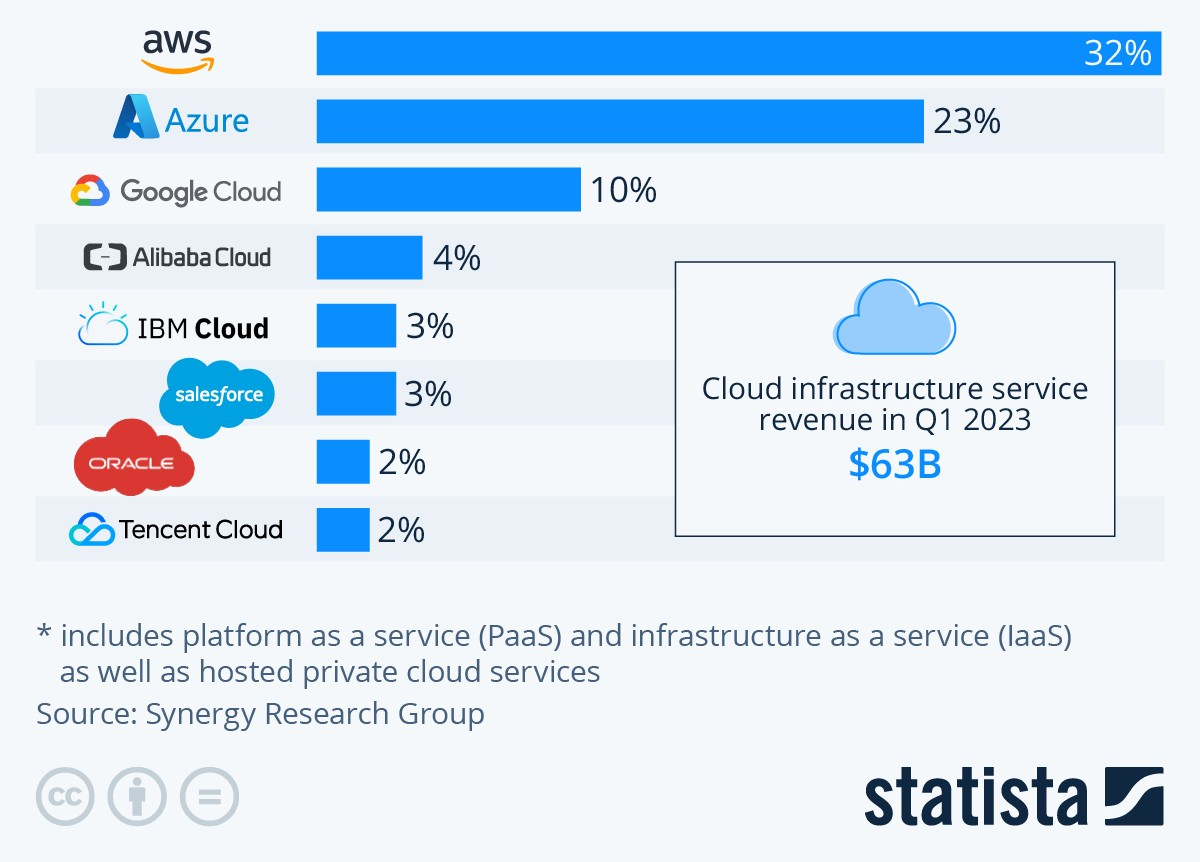
\includegraphics[width=\columnwidth]{Figures/Graphs/Cloud_market_share.jpeg}
\caption{Worldwide market share of leading cloud infrastructure providers in Q1 2023. Source: Statista}
\label{Cloud market share}
\end{figure}

\subsection{Local machine}
With the prospect of using cloud infrastructure seeming slim, we turned to doing what we could with the resources available to us. We both possessed personal desktop computers with decent processing power. 
Running on a local machine would give much better control over the system, and the project would not be beholden to the whims of a cloud service provider. 
It does come with some drawbacks. Microservices are a cloud focused architecture type. Data generated from a local machine it is much less likely to be directly relatable to real world systems that might make use of the research.

There are a variety of tools that help launch containers for microservices locally. Most of them are a subset or extension of Docker. 

\subsection{Candidates}
\subsubsection{DeathStarBench}
DeathStarBench is an open-source benchmark suite developed by Cornell University for research purposes. 
It features a total of five complete services: A social network, a media service, hotel reservation, an e-commerce site, a banking system, and a drone coordination system for drone swarms. If chosen as the system for this project, we would have focused on one of the first three services. They are in a more complete state than the rest according to the project's GitHub page. 
DeathStarBench makes a compelling choice as it seems to be quite complete and sophisticated, as well as being made specifically for testing. \cite*{Gan2019} \\
However, there were two main issues with it.
\begin{itemize}
    \item System requirements and complexity
\end{itemize}
The complex nature of the project made it unclear if we would be able to run it on our available hardware. There were also doubts as to how simple it would be to get up and running in the first place. We would run the risk of spending a lot of time getting it up and running, only to find that it doesn't have enough resources to run properly.
\begin{figure}[ht]
\centering 
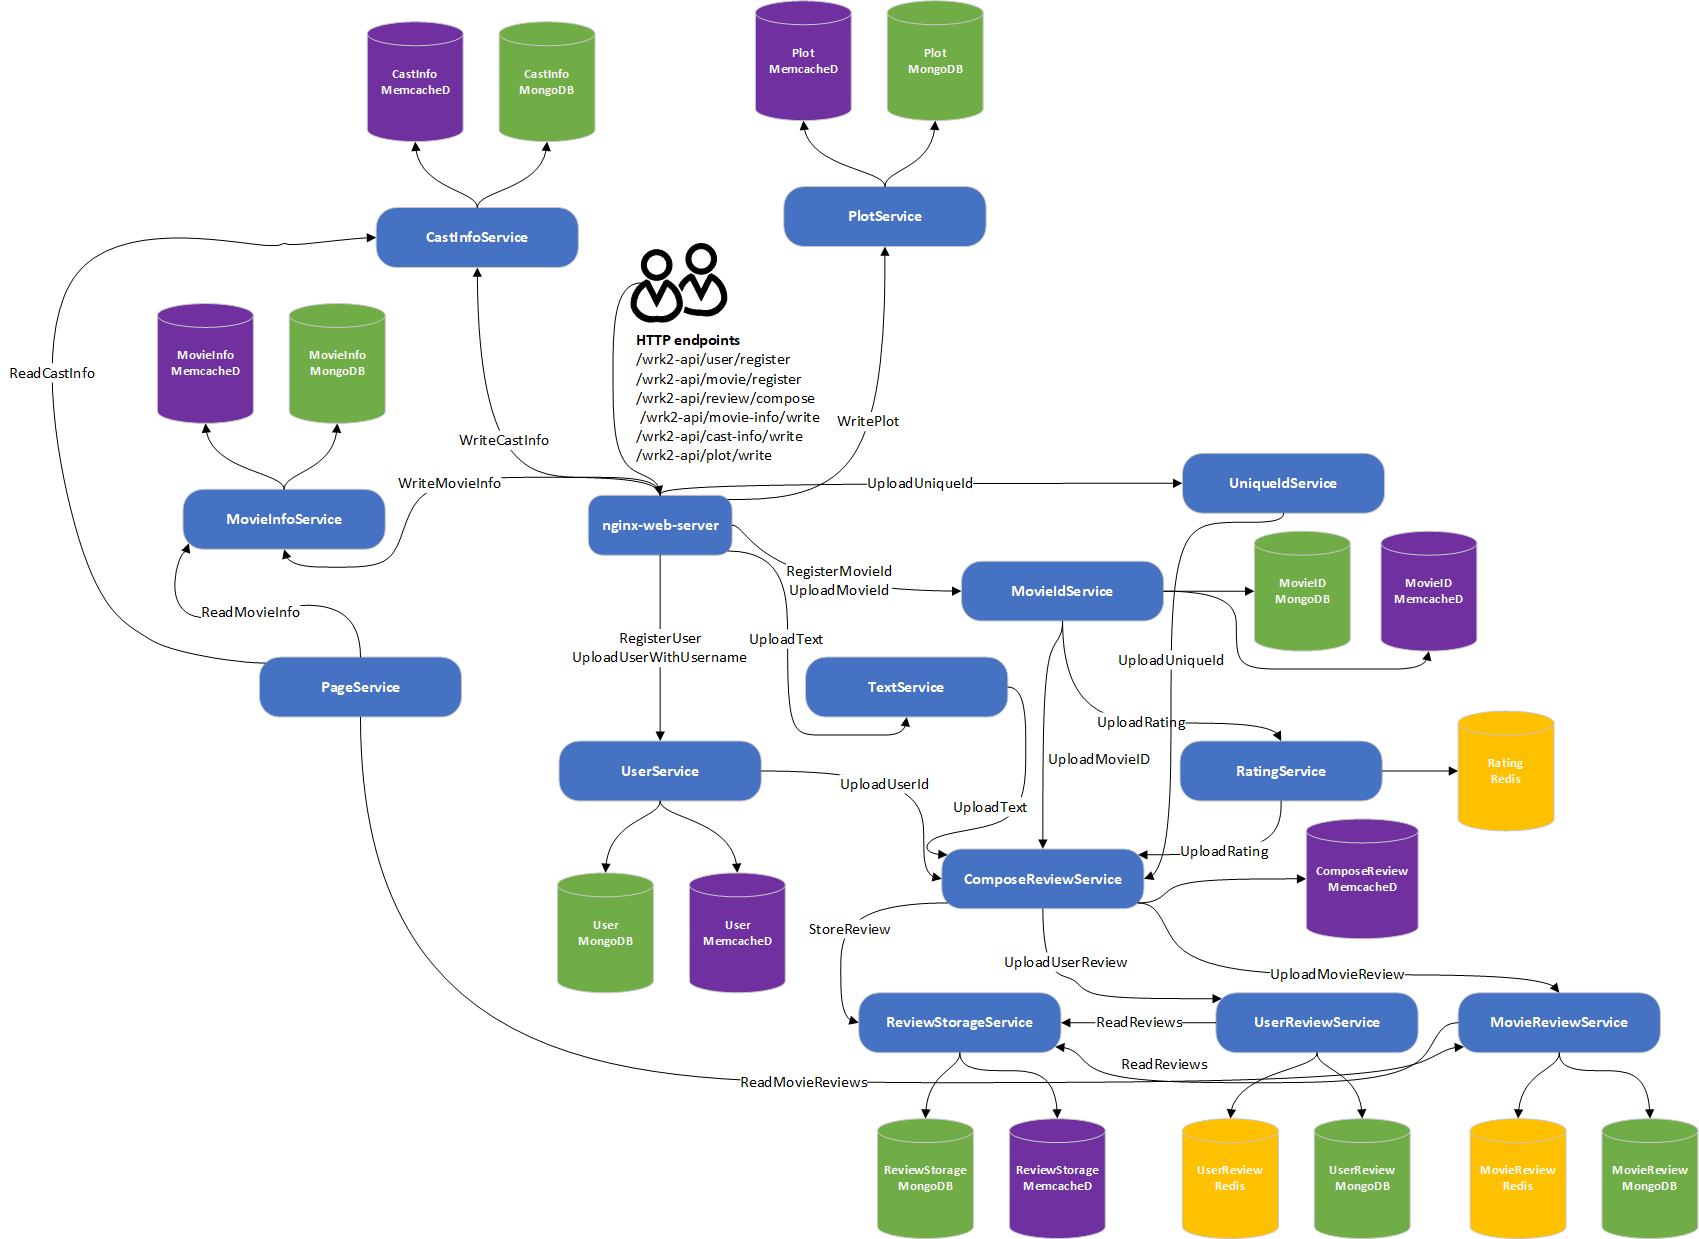
\includegraphics[width=\columnwidth]{Figures/Charts/media_microservices_architecture.png}
\caption{The workload architecture for DSB's media service}
\label{DSB-media}
\end{figure}
\begin{itemize}
    \item Distributed tracing
\end{itemize}
DeathStarBench uses Jaeger to provide distributed tracing of the system. This provides detailed information about the behavior of the system during operation. Higher quality data lets ML models train more efficiently and provide more accurate and detailed results. 
Working with this would put the focus of the project work into the realm of making use of the data for more detailed prediction purposes, something that is already quite thoroughly studied by people with more skills and resources. \cite*{Bogatinovski}, \cite*{Nedelkoski2019}, \cite*{Zhou2021a}



\subsubsection{Sockshop}
Sockshop is a lightweight microservices demo created by Weaveworks inc. It is "intended to aid the demonstration and testing of microservice and cloud native technologies". \cite*{Weaveworks} It simulates an online sock retailer, complete with users, carts, catalogs etc. 
It is an older, smaller project, and parts of it were used to build the larger DeathStarBench. \cite*{Gan2019}
The smaller, less complex nature of this project means that it could feasibly run on our available home machines. 
It is composed of 14 services running in individual containers. The messaging between them is handled by RabbitMQ, which runs as its own container as one of the 14. 

\begin{figure}[ht] 
\centering 
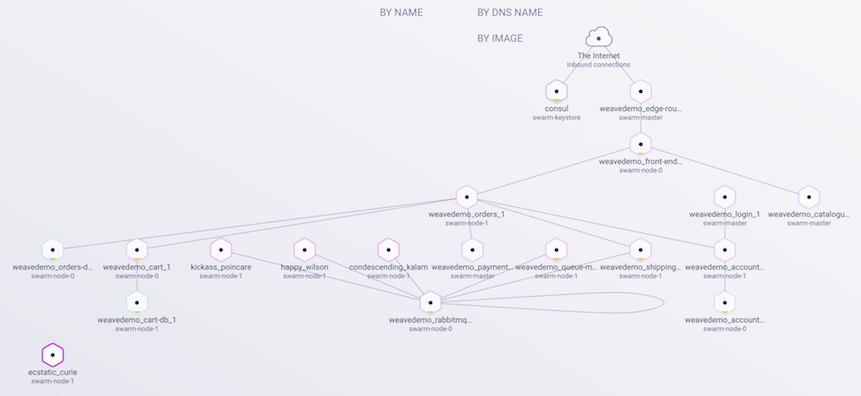
\includegraphics[width=\columnwidth]{Figures/Charts/sockshop-scope_trimmed.png}
\caption{The architecture of the sock shop shown using WeaveScope, Weaveworks' own mapping tool.}
\label{Sockshop architecture}
\end{figure}

Sockshop comes with some strong benefits:

\begin{itemize}
    \item Forgiving system requirements
\end{itemize}

Of the strong candidates, this was the one most likely to not run into a hardware bottleneck on our computers. 

\begin{itemize}
    \item Centralized logging
\end{itemize}
Sockshop comes instrumented with Prometheus, and publishes an API endpoint for retrieving metrics from the Prometheus microservice. Centralized logging provides less insight than distributed tracing, but carries less resource overhead and is easier to add to an existing system, since it is less invasive. 
This provides an angle to give a unique value proposition to the project: A method for learning about and optimizing an already existing system, while minimizing time and effort spent instrumenting the microservice system and training the models. Results would not be as accurate or reliable as more thorough projects using data collected from distributed tracing, but it could provide a "good enough" result for a fraction of the investment.

There are also some major downsides to the Sockshop.

\begin{itemize}
    \item Poor documentation
\end{itemize}
The website for the project \cite*{Weaveworks} has documentation, but it gives few details about the underlying structure of the system. 
For example, it has Prometheus instrumentation. But it gives no information on which client libraries are installed where. Finding out requires digging through the source code and metrics.
The project has been dead for some time. The last commit on GitHub as of time of writing was on August 17, 2021. 